%%%%%%%%%%%%%%%%%%%%%%%%%%%%%%%%%%%%%%%%%
% baposter Landscape Poster
% LaTeX Template
% Version 1.0 (11/06/13)
%
% baposter Class Created by:
% Brian Amberg (baposter@brian-amberg.de)
%
% This template has been downloaded from:
% http://www.LaTeXTemplates.com
%
% License:
% CC BY-NC-SA 3.0 (http://creativecommons.org/licenses/by-nc-sa/3.0/)
%
%%%%%%%%%%%%%%%%%%%%%%%%%%%%%%%%%%%%%%%%%

%----------------------------------------------------------------------------------------
%	PACKAGES AND OTHER DOCUMENT CONFIGURATIONS
%----------------------------------------------------------------------------------------

\documentclass[landscape,a0paper,fontscale=0.285]{baposter} % Adjust the font scale/size here

\usepackage{graphicx} % Required for including images
\graphicspath{{figures/}} % Directory in which figures are stored

\usepackage{amsmath} % For typesetting math
\usepackage{amssymb} % Adds new symbols to be used in math mode

\usepackage{booktabs} % Top and bottom rules for tables
\usepackage{enumitem} % Used to reduce itemize/enumerate spacing
\usepackage{palatino} % Use the Palatino font
\usepackage[font=small,labelfont=bf]{caption} % Required for specifying captions to tables and figures
\usepackage{hyperref}
\usepackage{caption}
\usepackage{multicol} % Required for multiple columns
\setlength{\columnsep}{1.5em} % Slightly increase the space between columns
\setlength{\columnseprule}{0mm} % No horizontal rule between columns
\usepackage{multirow}% http://ctan.org/pkg/multirow
\usepackage{hhline}% http://ctan.org/pkg/hhline
\usepackage{tikz} % Required for flow chart
\usepackage{amsmath}
\usepackage{graphicx}
\usepackage{bm}
\usetikzlibrary{shapes,arrows} % Tikz libraries required for the flow chart in the template

\newcommand{\compresslist}{ % Define a command to reduce spacing within itemize/enumerate environments, this is used right after \begin{itemize} or \begin{enumerate}
\setlength{\itemsep}{1pt}
\setlength{\parskip}{0pt}
\setlength{\parsep}{0pt}
}

\definecolor{lightblue}{rgb}{0.53,0.81,0.98} % Defines the color used for content box headers
\DeclareMathOperator*{\argmin}{arg\,min}

\begin{document}

\begin{poster}
{
headerborder=closed, % Adds a border around the header of content boxes
colspacing=1em, % Column spacing
bgColorOne=white, % Background color for the gradient on the left side of the poster
bgColorTwo=white, % Background color for the gradient on the right side of the poster
borderColor=lightblue, % Border color
headerColorOne=white, % Background color for the header in the content boxes (left side)
headerColorTwo=lightblue, % Background color for the header in the content boxes (right side)
headerFontColor=black, % Text color for the header text in the content boxes
boxColorOne=white, % Background color of the content boxes
textborder=roundedleft, % Format of the border around content boxes, can be: none, bars, coils, triangles, rectangle, rounded, roundedsmall, roundedright or faded
eyecatcher=true, % Set to false for ignoring the left logo in the title and move the title left
headerheight=0.1\textheight, % Height of the header
headershape=roundedright, % Specify the rounded corner in the content box headers, can be: rectangle, small-rounded, roundedright, roundedleft or rounded
headerfont=\Large\bf\textsc, % Large, bold and sans serif font in the headers of content boxes
%textfont={\setlength{\parindent}{1.5em}}, % Uncomment for paragraph indentation
linewidth=2pt % Width of the border lines around content boxes
}
%----------------------------------------------------------------------------------------
%	TITLE SECTION 
%----------------------------------------------------------------------------------------
%
{
\includegraphics[height=5em]{usc_logo.png}} % First university/lab logo on the left
{\bf\textsc{\huge High-Resolution Image Inpainting using Multi-Scale Neural Patch Synthesis}\vspace{.1em}} % Poster title
{\textsc{\{Chao ``Harry'' Yang, Xin Lu, Zhe Lin, Eli Schechtman, Oliver Wang and Hao Li\} \hspace{12pt} \parbox{0.3\textwidth}{\small *University of Southern California\\$^\dagger$Adobe Research}}} % Author names and institution
{
\includegraphics[height=5em]{adobe_logo.jpg}} 
%----------------------------------------------------------------------------------------
%	OBJECTIVES
%----------------------------------------------------------------------------------------

\headerbox{Bad Things Happen}{name=objectives,column=0,span=1, row=0}{
\begin{minipage}[t]{1\linewidth}
\begin{center}
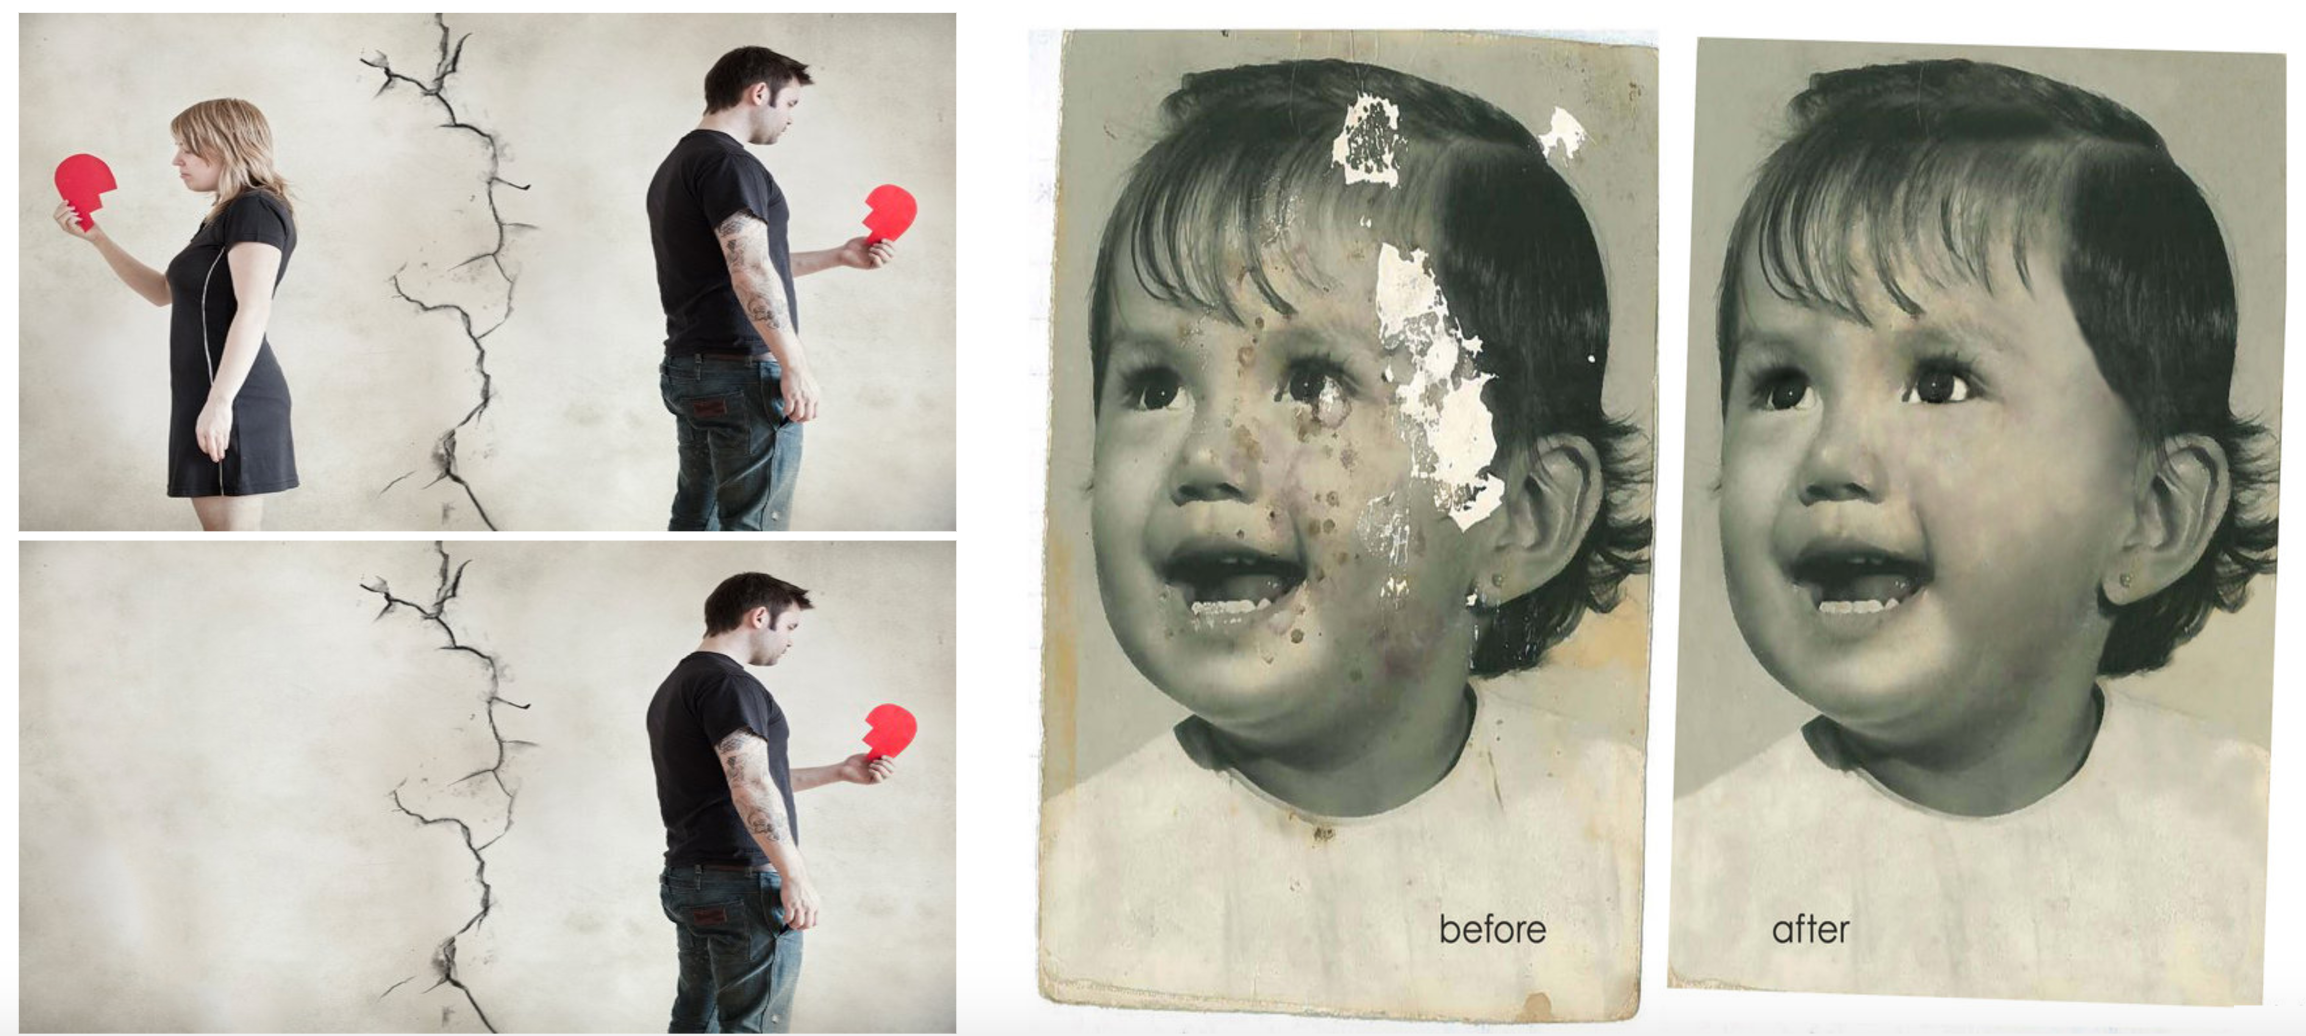
\includegraphics[width=1\columnwidth]{figures/problem.png}
\end{center}
\end{minipage}
Imaging you would like to edit a photo after breaking up, or restore an old picture from damages, we designed a MULTI-SCALE DEEP LEARNING algorithm to help you! We
\begin{itemize}
\item proposed a joint optimization framework that can hallucinates missing image regions by modeling a global content constraint and local texture constraint with convolutional neural networks.
\item further introduced a multi-scale neural patch syn- thesis algorithm for high-resolution image inpainting based on the joint optimization framework.
\end{itemize}
\vspace{0.3em} % When there are two boxes, some whitespace may need to be added if the one on the right has more content
}

%----------------------------------------------------------------------------------------
%	INTRODUCTION
%----------------------------------------------------------------------------------------

\headerbox{The Content Network}{name=content,column=1,span=1, row=0}{
\begin{minipage}{1\linewidth}
\begin{minipage}[t]{1\linewidth}
\begin{center}
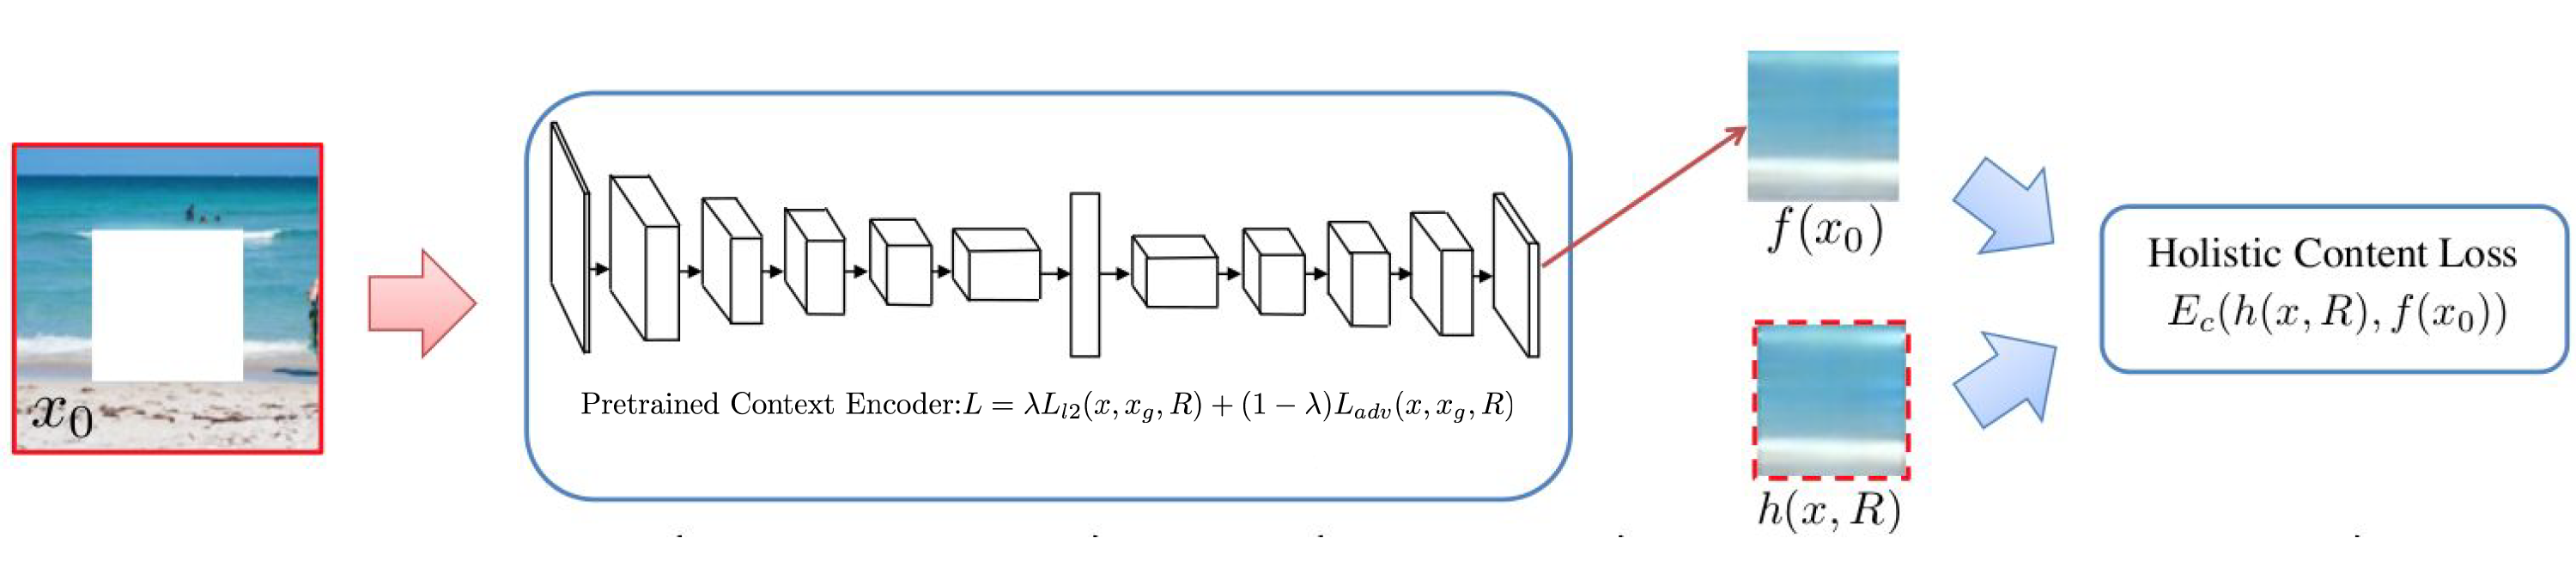
\includegraphics[width=1\columnwidth]{figures/content_network.png}
\end{center}
\end{minipage}
\begin{center}
\noindent\textbf{Context Encoder Predicts the Low-Res Content}
\end{center}
The content constraint: 
\begin{equation}
E_c(h(x,R), h(x_i,R))  = \parallel h(x,R) - h(x_i,R) \parallel_2^2
\end{equation}
\end{minipage}
}

\headerbox{The Texture Network}{name=texture,column=1,span=1, below=content}{
\begin{minipage}{1\linewidth}
\begin{minipage}[t]{1\linewidth}
\begin{center}
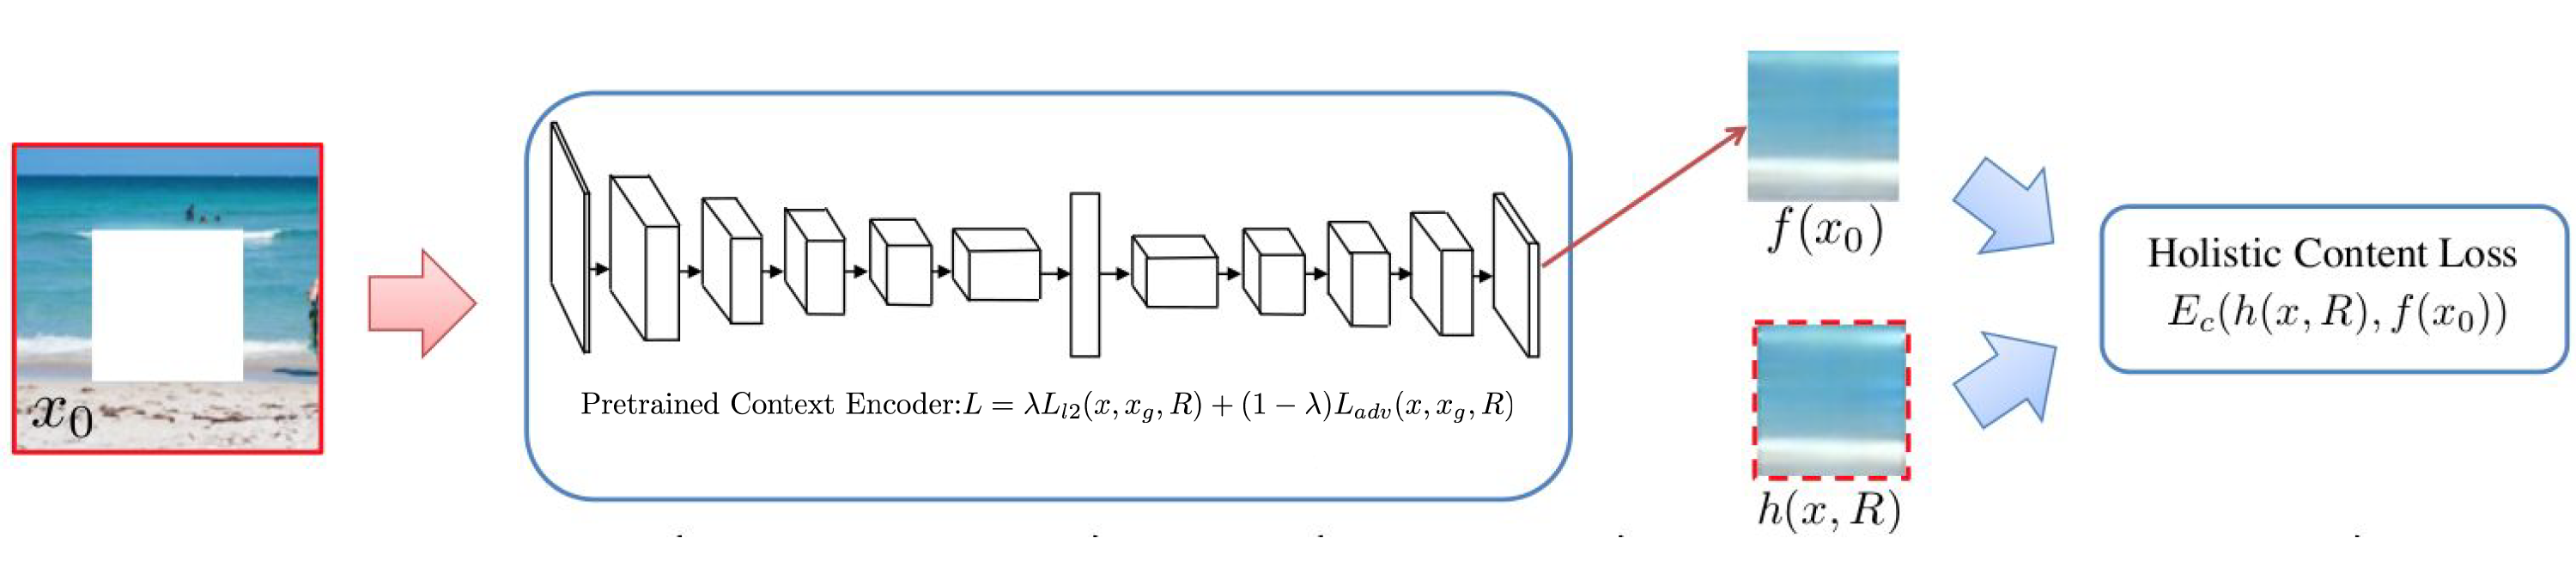
\includegraphics[width=1\columnwidth]{figures/content_network.png}
\end{center}
\end{minipage}
\begin{center}
\noindent\textbf{Pre-trained VGG Optimizes the High-Res Texture}
\end{center}
The texture constraint:
\begin{multline}
E_t(\phi_t(x),R)  = \\ 
\frac{1}{|R^{\phi}|}\sum_{i\in R^{\phi}} \parallel h(\phi_t(x),P_i) - h(\phi_t(x),P_{nn(i)})  \parallel_2^2
\end{multline}
\end{minipage}
}

\headerbox{The Joint Loss Function}{name=loss,column=1,span=1,below=texture}{
At each iteration, we minimize:\\
\begin{minipage}{1\linewidth}
\begin{eqnarray*}
\tilde{x}_{i+1} = && \argmin_{x} E_c(h(x,R), h(x_i,R)) \nonumber \\ 
&& +\alpha E_t(\phi_t(x),R^{\phi})  + \beta \Upsilon(x)
\label{eq:opt}
\end{eqnarray*}
\end{minipage}
}

\headerbox{Multi-scale Optimization}{name=multiscale,column=1,span=1, below=loss}{
We optimize at three scales: 128, 256 and 512:
\begin{minipage}{1\linewidth}
\begin{minipage}[t]{1\linewidth}
\begin{center}
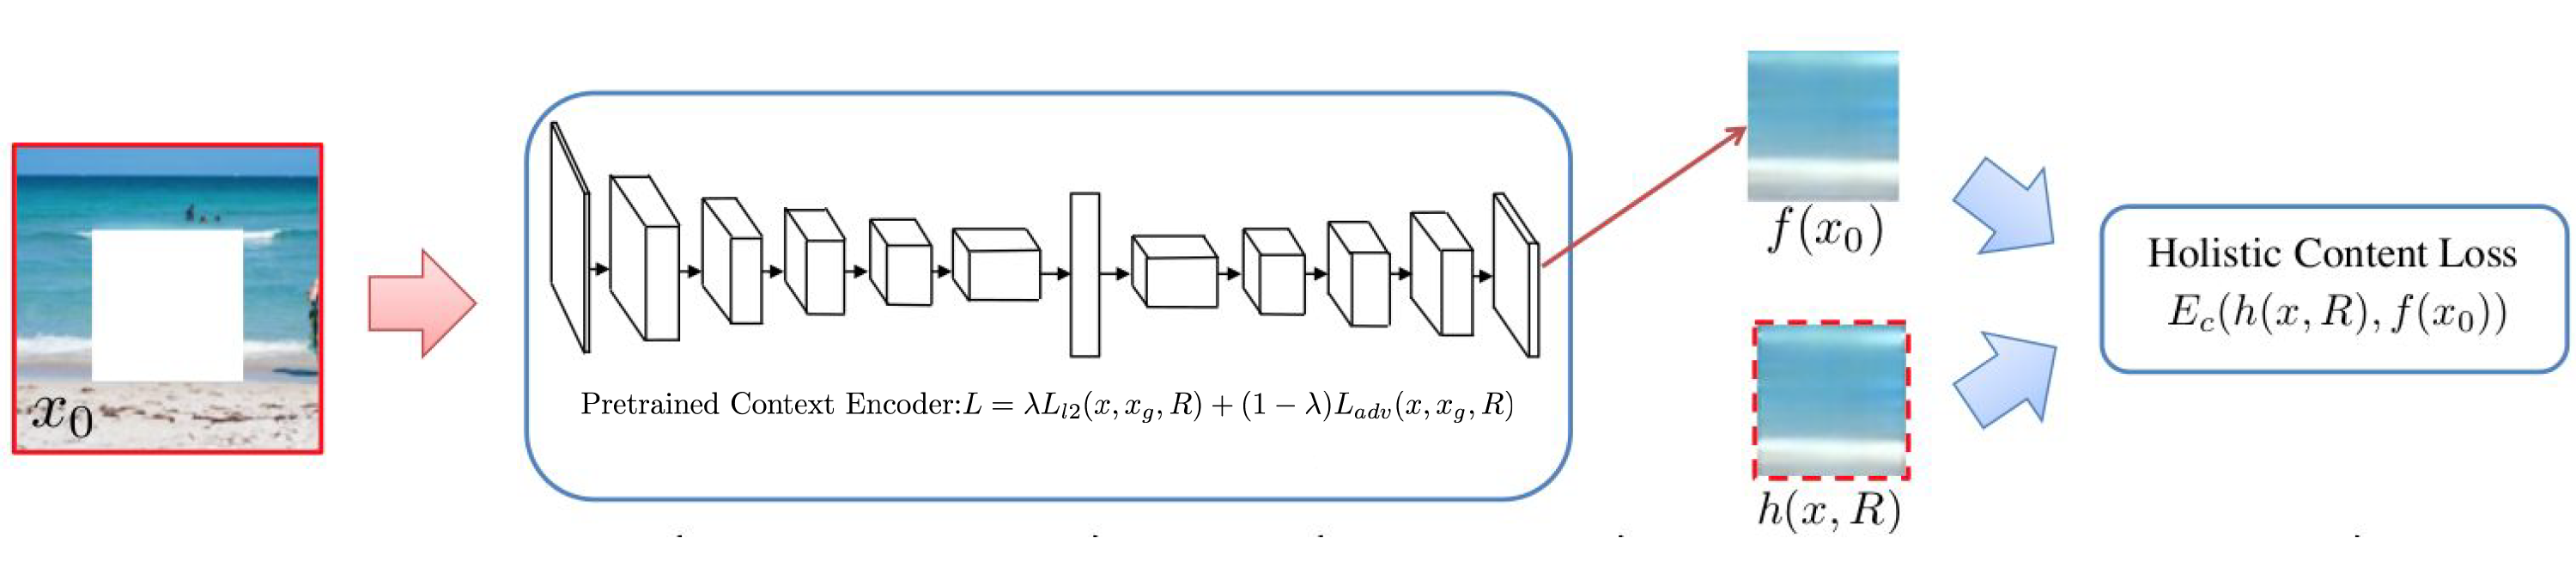
\includegraphics[width=1\columnwidth]{figures/content_network.png}
\end{center}
\end{minipage}
\begin{center}
\noindent\textbf{Pre-trained VGG: Optimizing the high-res texture}
\end{center}
\end{minipage}
}


\headerbox{Changing the Weight $\alpha$}{name=weight,column=2,span=1, row=0}{ % This block's bottom aligns with the bottom of the conclusion block
The weight $\alpha$ measures the contribution of the texture constraint relative to the content constraint. It is a trade off between the sharpness of the texture and coherence of the structure: 
\begin{figure}[h!]
\setlength\tabcolsep{1.5pt}
\centering
\small
\begin{tabular}{cccc}
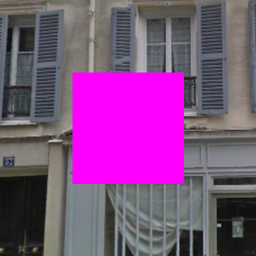
\includegraphics[width=.24\linewidth]{figures/pink_0046_r.png} &
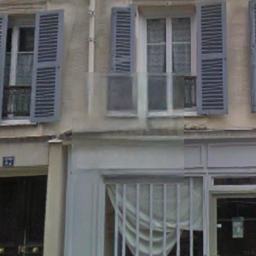
\includegraphics[width=.24\linewidth]{figures/res_3_100_1_r.png} &
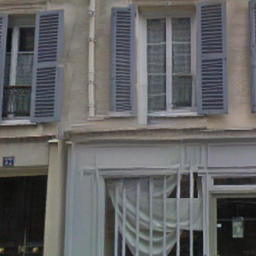
\includegraphics[width=.24\linewidth]{figures/res_3_100_2_r.png} &
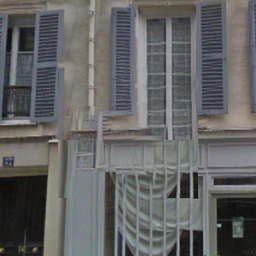
\includegraphics[width=.24\linewidth]{figures/res_3_100_3_r.png} \\
(a) Input image & (b) $\alpha=1e-6$ & (c) $\alpha=1e-5$ & (d) $\alpha=4e-5$\\ 
\end{tabular}
%\caption{The effect of texture weight $\alpha$. }\label{alpha}
\end{figure} 
}

\headerbox{Dropping the content constraint}{name=drop_content,column=2,span=1, below=weight }{ % This block's bottom aligns with the bottom of the conclusion block
The weight $\alpha$ measures the contribution of the texture constraint relative to the content constraint. It is a trade off between the sharpness of the texture and coherence of the structure: 
\begin{figure}[h!]
\setlength\tabcolsep{1.5pt}
\centering
\small
\begin{tabular}{cccc}
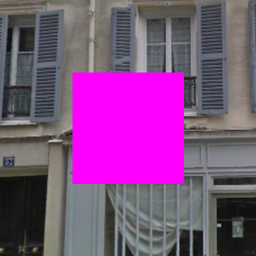
\includegraphics[width=.24\linewidth]{figures/pink_0046_r.png} &
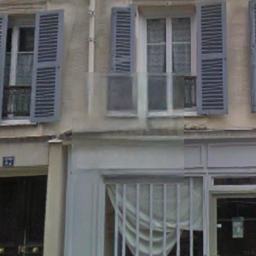
\includegraphics[width=.24\linewidth]{figures/res_3_100_1_r.png} &
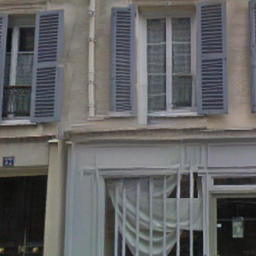
\includegraphics[width=.24\linewidth]{figures/res_3_100_2_r.png} &
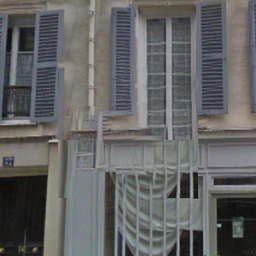
\includegraphics[width=.24\linewidth]{figures/res_3_100_3_r.png} \\
(a) Input image & (b) $\alpha=1e-6$ & (c) $\alpha=1e-5$ & (d) $\alpha=4e-5$\\ 
\end{tabular}
%\caption{The effect of texture weight $\alpha$. }\label{alpha}
\end{figure} 
}

\headerbox{Dropping the adversarial loss}{name=drop_adversarial,column=2,span=1, below=drop_content}{ % This block's bottom aligns with the bottom of the conclusion block
The weight $\alpha$ measures the contribution of the texture constraint relative to the content constraint. It is a trade off between the sharpness of the texture and coherence of the structure: 
\begin{figure}[h!]
\setlength\tabcolsep{1.5pt}
\centering
\small
\begin{tabular}{cccc}
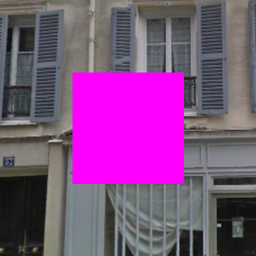
\includegraphics[width=.24\linewidth]{figures/pink_0046_r.png} &
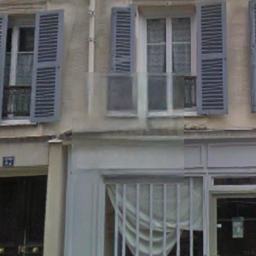
\includegraphics[width=.24\linewidth]{figures/res_3_100_1_r.png} &
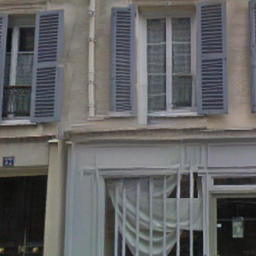
\includegraphics[width=.24\linewidth]{figures/res_3_100_2_r.png} &
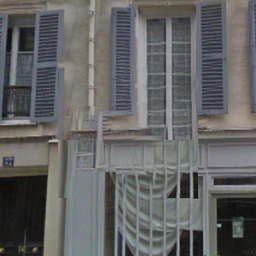
\includegraphics[width=.24\linewidth]{figures/res_3_100_3_r.png} \\
(a) Input image & (b) $\alpha=1e-6$ & (c) $\alpha=1e-5$ & (d) $\alpha=4e-5$\\ 
\end{tabular}
%\caption{The effect of texture weight $\alpha$. }\label{alpha}
\end{figure} 
}

\headerbox{Comparison}{name=drop_adversarial,column=2,span=1, below=drop_adversarial}{ % This block's bottom aligns with the bottom of the conclusion block
The weight $\alpha$ measures the contribution of the texture constraint relative to the content constraint. It is a trade off between the sharpness of the texture and coherence of the structure: 
\begin{figure}[h!]
\setlength\tabcolsep{1.5pt}
\centering
\small
\begin{tabular}{cccc}
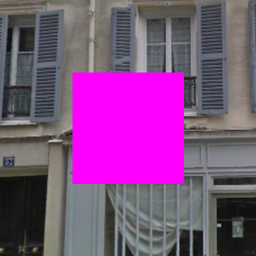
\includegraphics[width=.24\linewidth]{figures/pink_0046_r.png} &
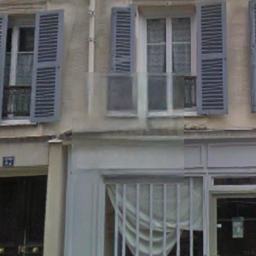
\includegraphics[width=.24\linewidth]{figures/res_3_100_1_r.png} &
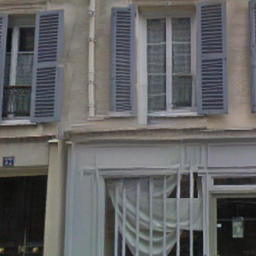
\includegraphics[width=.24\linewidth]{figures/res_3_100_2_r.png} &
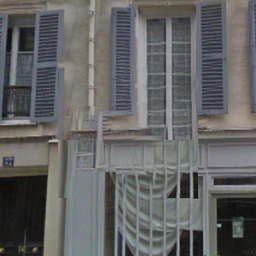
\includegraphics[width=.24\linewidth]{figures/res_3_100_3_r.png} \\
(a) Input image & (b) $\alpha=1e-6$ & (c) $\alpha=1e-5$ & (d) $\alpha=4e-5$\\ 
\end{tabular}
%\caption{The effect of texture weight $\alpha$. }\label{alpha}
\end{figure} 
}

\headerbox{Result on ImageNet}{name=imagenet,column=3,span=1, row=0}{ % This block's bottom aligns with the bottom of the conclusion block
The weight $\alpha$ measures the contribution of the texture constraint relative to the content constraint. It is a trade off between the sharpness of the texture and coherence of the structure: 
\begin{figure}[h!]
\setlength\tabcolsep{1.5pt}
\centering
\small
\begin{tabular}{cccc}
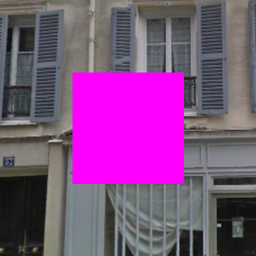
\includegraphics[width=.24\linewidth]{figures/pink_0046_r.png} &
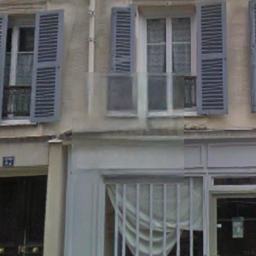
\includegraphics[width=.24\linewidth]{figures/res_3_100_1_r.png} &
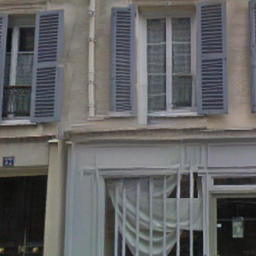
\includegraphics[width=.24\linewidth]{figures/res_3_100_2_r.png} &
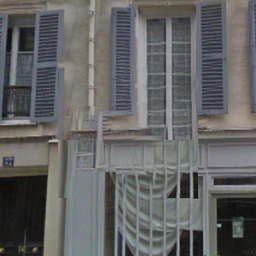
\includegraphics[width=.24\linewidth]{figures/res_3_100_3_r.png} \\
(a) Input image & (b) $\alpha=1e-6$ & (c) $\alpha=1e-5$ & (d) $\alpha=4e-5$\\ 
\end{tabular}
%\caption{The effect of texture weight $\alpha$. }\label{alpha}
\end{figure} 
}


\headerbox{Result on Paris Streetview}{name=paris,column=3,span=1, below=imagenet}{ % This block's bottom aligns with the bottom of the conclusion block
The weight $\alpha$ measures the contribution of the texture constraint relative to the content constraint. It is a trade off between the sharpness of the texture and coherence of the structure: 
\begin{figure}[h!]
\setlength\tabcolsep{1.5pt}
\centering
\small
\begin{tabular}{cccc}
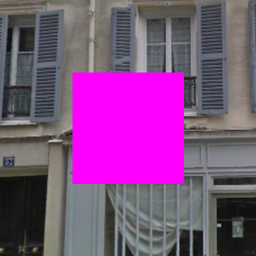
\includegraphics[width=.24\linewidth]{figures/pink_0046_r.png} &
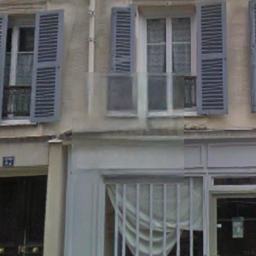
\includegraphics[width=.24\linewidth]{figures/res_3_100_1_r.png} &
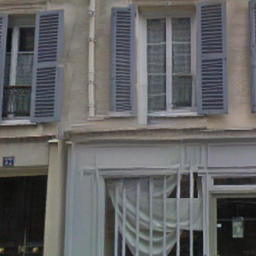
\includegraphics[width=.24\linewidth]{figures/res_3_100_2_r.png} &
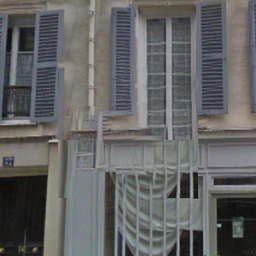
\includegraphics[width=.24\linewidth]{figures/res_3_100_3_r.png} \\
(a) Input image & (b) $\alpha=1e-6$ & (c) $\alpha=1e-5$ & (d) $\alpha=4e-5$\\ 
\end{tabular}
%\caption{The effect of texture weight $\alpha$. }\label{alpha}
\end{figure} 
}

\headerbox{Result on Arbitrary Shape}{name=arbitrary,column=3,span=1, below=paris}{ % This block's bottom aligns with the bottom of the conclusion block
The weight $\alpha$ measures the contribution of the texture constraint relative to the content constraint. It is a trade off between the sharpness of the texture and coherence of the structure: 
\begin{figure}[h!]
\setlength\tabcolsep{1.5pt}
\centering
\small
\begin{tabular}{cccc}
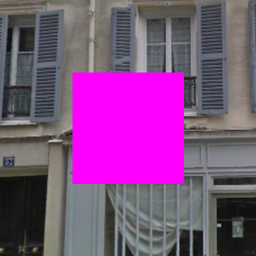
\includegraphics[width=.24\linewidth]{figures/pink_0046_r.png} &
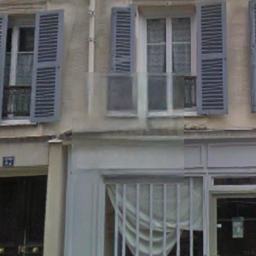
\includegraphics[width=.24\linewidth]{figures/res_3_100_1_r.png} &
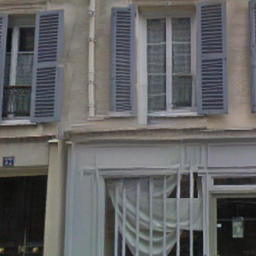
\includegraphics[width=.24\linewidth]{figures/res_3_100_2_r.png} &
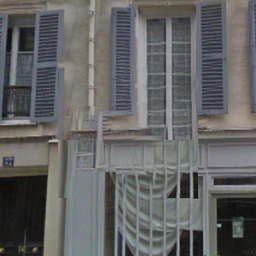
\includegraphics[width=.24\linewidth]{figures/res_3_100_3_r.png} \\
(a) Input image & (b) $\alpha=1e-6$ & (c) $\alpha=1e-5$ & (d) $\alpha=4e-5$\\ 
\end{tabular}
%\caption{The effect of texture weight $\alpha$. }\label{alpha}
\end{figure} 
}

\headerbox{Code and Supplementary Material}{name=code,column=3, span=1, below=arbitrary}{ % This block's bottom aligns with the bottom of the conclusion block
Code is available at \href{www.harryyang.org/inpainting}www.harryyang.org/inpainting
}

\headerbox{Algorithm}{name=algorithm,column=0, below=objectives}{ % This block's bottom aligns with the bottom of the conclusion block
test
}


%----------------------------------------------------------------------------------------

\end{poster}

\end{document}